\documentclass[12pt]{beamer}\usepackage[]{graphicx}\usepackage[]{color}
%% maxwidth is the original width if it is less than linewidth
%% otherwise use linewidth (to make sure the graphics do not exceed the margin)
\makeatletter
\def\maxwidth{ %
  \ifdim\Gin@nat@width>\linewidth
    \linewidth
  \else
    \Gin@nat@width
  \fi
}
\makeatother

\definecolor{fgcolor}{rgb}{0.345, 0.345, 0.345}
\newcommand{\hlnum}[1]{\textcolor[rgb]{0.686,0.059,0.569}{#1}}%
\newcommand{\hlstr}[1]{\textcolor[rgb]{0.192,0.494,0.8}{#1}}%
\newcommand{\hlcom}[1]{\textcolor[rgb]{0.678,0.584,0.686}{\textit{#1}}}%
\newcommand{\hlopt}[1]{\textcolor[rgb]{0,0,0}{#1}}%
\newcommand{\hlstd}[1]{\textcolor[rgb]{0.345,0.345,0.345}{#1}}%
\newcommand{\hlkwa}[1]{\textcolor[rgb]{0.161,0.373,0.58}{\textbf{#1}}}%
\newcommand{\hlkwb}[1]{\textcolor[rgb]{0.69,0.353,0.396}{#1}}%
\newcommand{\hlkwc}[1]{\textcolor[rgb]{0.333,0.667,0.333}{#1}}%
\newcommand{\hlkwd}[1]{\textcolor[rgb]{0.737,0.353,0.396}{\textbf{#1}}}%

\usepackage{framed}
\makeatletter
\newenvironment{kframe}{%
 \def\at@end@of@kframe{}%
 \ifinner\ifhmode%
  \def\at@end@of@kframe{\end{minipage}}%
  \begin{minipage}{\columnwidth}%
 \fi\fi%
 \def\FrameCommand##1{\hskip\@totalleftmargin \hskip-\fboxsep
 \colorbox{shadecolor}{##1}\hskip-\fboxsep
     % There is no \\@totalrightmargin, so:
     \hskip-\linewidth \hskip-\@totalleftmargin \hskip\columnwidth}%
 \MakeFramed {\advance\hsize-\width
   \@totalleftmargin\z@ \linewidth\hsize
   \@setminipage}}%
 {\par\unskip\endMakeFramed%
 \at@end@of@kframe}
\makeatother

\definecolor{shadecolor}{rgb}{.97, .97, .97}
\definecolor{messagecolor}{rgb}{0, 0, 0}
\definecolor{warningcolor}{rgb}{1, 0, 1}
\definecolor{errorcolor}{rgb}{1, 0, 0}
\newenvironment{knitrout}{}{} % an empty environment to be redefined in TeX

\usepackage{alltt}
\usepackage{graphicx}
\usepackage{tikz}
\setbeameroption{hide notes}
\setbeamertemplate{note page}[plain]
\usepackage{listings}

% get rid of junk
\usetheme{default}
\usefonttheme[onlymath]{serif}
\beamertemplatenavigationsymbolsempty
\hypersetup{pdfpagemode=UseNone} % don't show bookmarks on initial view

% named colors
\definecolor{offwhite}{RGB}{255,250,240}
\definecolor{gray}{RGB}{155,155,155}

\ifx\notescolors\undefined % slides

  \definecolor{foreground}{RGB}{80,80,80}
  \definecolor{background}{RGB}{255,255,255}
  \definecolor{title}{RGB}{255,199,0}
  \definecolor{subtitle}{RGB}{89,132,212}
  \definecolor{hilit}{RGB}{248,117,79}
  \definecolor{vhilit}{RGB}{255,111,207}
  \definecolor{lolit}{RGB}{200,200,200}
  \definecolor{lit}{RGB}{255,199,0}
  \definecolor{mdlit}{RGB}{89,132,212}
  \definecolor{link}{RGB}{248,117,79}

\else % notes
  \definecolor{background}{RGB}{255,255,255}
  \definecolor{foreground}{RGB}{24,24,24}
  \definecolor{title}{RGB}{27,94,134}
  \definecolor{subtitle}{RGB}{22,175,124}
  \definecolor{hilit}{RGB}{122,0,128}
  \definecolor{vhilit}{RGB}{255,0,128}
  \definecolor{lolit}{RGB}{95,95,95}
\fi
\definecolor{nhilit}{RGB}{128,0,128}  % hilit color in notes
\definecolor{nvhilit}{RGB}{255,0,128} % vhilit for notes

\newcommand{\hilit}{\color{hilit}}
\newcommand{\vhilit}{\color{vhilit}}
\newcommand{\nhilit}{\color{nhilit}}
\newcommand{\nvhilit}{\color{nvhilit}}
\newcommand{\lit}{\color{lit}}
\newcommand{\mdlit}{\color{mdlit}}
\newcommand{\lolit}{\color{lolit}}

% use those colors
\setbeamercolor{titlelike}{fg=title}
\setbeamercolor{subtitle}{fg=subtitle}
\setbeamercolor{frametitle}{fg=gray}
\setbeamercolor{structure}{fg=subtitle}
\setbeamercolor{institute}{fg=lolit}
\setbeamercolor{normal text}{fg=foreground,bg=background}
%\setbeamercolor{item}{fg=foreground} % color of bullets
%\setbeamercolor{subitem}{fg=hilit}
%\setbeamercolor{itemize/enumerate subbody}{fg=lolit}
\setbeamertemplate{itemize subitem}{{\textendash}}
\setbeamerfont{itemize/enumerate subbody}{size=\footnotesize}
\setbeamerfont{itemize/enumerate subitem}{size=\footnotesize}

% center title of slides
\setbeamertemplate{blocks}[rounded]
\setbeamertemplate{frametitle}[default][center]
% margins
\setbeamersize{text margin left=25pt,text margin right=25pt}

% page number
\setbeamertemplate{footline}{%
    \raisebox{5pt}{\makebox[\paperwidth]{\hfill\makebox[20pt]{\lolit
          \scriptsize\insertframenumber}}}\hspace*{5pt}}

% add a bit of space at the top of the notes page
\addtobeamertemplate{note page}{\setlength{\parskip}{12pt}}

% default link color
\hypersetup{colorlinks, urlcolor={link}}

\ifx\notescolors\undefined % slides
  % set up listing environment
  \lstset{language=bash,
          basicstyle=\ttfamily\scriptsize,
          frame=single,
          commentstyle=,
          backgroundcolor=\color{darkgray},
          showspaces=false,
          showstringspaces=false
          }
\else % notes
  \lstset{language=bash,
          basicstyle=\ttfamily\scriptsize,
          frame=single,
          commentstyle=,
          backgroundcolor=\color{offwhite},
          showspaces=false,
          showstringspaces=false
          }
\fi

% a few macros
\newcommand{\code}[1]{\texttt{#1}}
\newcommand{\hicode}[1]{{\hilit \texttt{#1}}}
\newcommand{\bb}[1]{\begin{block}{#1}}
\newcommand{\eb}{\end{block}}
\newcommand{\bi}{\begin{itemize}}
%\newcommand{\bbi}{\vspace{24pt} \begin{itemize} \itemsep8pt}
\newcommand{\bbi}{\vspace{4pt} \begin{itemize} \itemsep8pt}
\newcommand{\ei}{\end{itemize}}
\newcommand{\bv}{\begin{verbatim}}
\newcommand{\ev}{\end{verbatim}}
\newcommand{\ig}{\includegraphics}
\newcommand{\subt}[1]{{\footnotesize \color{subtitle} {#1}}}
\newcommand{\ttsm}{\tt \small}
\newcommand{\ttfn}{\tt \footnotesize}
\newcommand{\figh}[2]{\centerline{\includegraphics[height=#2\textheight]{#1}}}
\newcommand{\figw}[2]{\centerline{\includegraphics[width=#2\textwidth]{#1}}}



%------------------------------------------------
% end of header
%------------------------------------------------

\title{Simulation - part 1}
\subtitle{STAT 133}
\author{\href{http://www.gastonsanchez.com}{Gaston Sanchez}}
\institute{Department of Statistics, UC{\textendash}Berkeley}
\date{\href{http://www.gastonsanchez.com}{\tt \scriptsize \color{foreground} gastonsanchez.com}
\\[-4pt]
\href{http://github.com/gastonstat/stat133}{\tt \scriptsize \color{foreground} github.com/gastonstat/stat133}
\\[-4pt]
{\scriptsize Course web: \href{http://www.gastonsanchez.com/stat133}{\tt gastonsanchez.com/stat133}}
}
\IfFileExists{upquote.sty}{\usepackage{upquote}}{}
\begin{document}


{
  \setbeamertemplate{footline}{} % no page number here
  \frame{
    \titlepage
  } 
}

%------------------------------------------------

\begin{frame}
\begin{center}
\Huge{\mdlit{How do we use a computer to simulate a chance process?}}
\end{center}
\end{frame}

%------------------------------------------------

\begin{frame}
\begin{center}
\Huge{\hilit{Case Study}}
\end{center}
\end{frame}

%------------------------------------------------

\begin{frame}
\frametitle{Chevalier de Mere}

\bbi
  \item Antoine Gombaud (1607 - 1684)
  \item \textit{Nom de plume} ``Chevalier de Mere''
  \item French writer and gambler, but not a nobleman
  \item Amateur mathematician
\ei

\end{frame}

%------------------------------------------------

\begin{frame}[fragile]
\frametitle{}
\begin{center}
\ig[width=5cm]{images/dice4.jpg}
\end{center}
\end{frame}

%------------------------------------------------

\begin{frame}[fragile]
\frametitle{De Mere's games}

\begin{columns}[t]
\begin{column}{0.4\textwidth}
Game 1
\bi
  \item One die
  \item Four rolls
  \item Win: at least one 6
\ei
\end{column}

\pause

\begin{column}{0.55\textwidth}
Game 2
\bi
  \item Two dice
  \item 24 rolls
  \item Win: at least one double 6
\ei
\end{column}
\end{columns}

\bigskip
\bigskip
\pause
De Mere was making money with game 1, but losing money with game 2. He turned to Blaise Pascal for help.
\end{frame}

%------------------------------------------------

\begin{frame}
\frametitle{De Mere's faulty reasoning}

\bb{Game 1}
\bbi
  \item The chance of getting a six in one roll of a die is $\frac{1}{6}$.
  \item In four rolls of a die, the chance of getting one six would be $\frac{4}{6}=\frac{2}{3}$.
\ei
\eb

\end{frame}

%------------------------------------------------

\begin{frame}
\frametitle{De Mere's faulty reasoning}

\bb{Game 2}
\bbi
  \item The chance of getting a double six in rolling a pair of dice is $\frac{1}{36}$.
  \item In 24 rolls of a pair of dice, the chance of getting one double six would be $\frac{24}{36}=\frac{2}{3}$.
\ei
\eb

\end{frame}

%------------------------------------------------

\begin{frame}
\frametitle{Pascal and Fermat}

\bbi
  \item De Mere turned into Blaise Pascal
  \item Pascal consulted with Pierre de Fermat
  \item Beginning of Pascal's and Fermat's famous correspondence (1650's)
  \item Origin of combinatorial probability
\ei

\end{frame}

%------------------------------------------------

\begin{frame}[fragile]
\frametitle{}
\begin{center}
\ig[width=11cm]{images/pascal_fermat.pdf}
\end{center}
\end{frame}

%------------------------------------------------

\begin{frame}
\frametitle{Letter from Pascal to Fermat}

\begin{quotation}
``If one undertakes to throw a six with one die, the advatange of undertaking it in 4 throws is as 671 to 625. If one undertakes to throw a double-six with two dice, there is a disadvantage of undertaking it in 24 throws. And nevertheless 24 is to 36 (which is the number of faces of two dice) as 4 to 6 (which is the number of faces of one die).''
\end{quotation}

\end{frame}

%------------------------------------------------

\begin{frame}[fragile]
\frametitle{De Mere's Game 1}

Probability of no six in four rolls:
$$
\frac{5}{6} \times \frac{5}{6} \times \frac{5}{6} \times \frac{5}{6} = \frac{625}{1296} = 0.482253
$$

\bigskip
\pause
P(at least one six) = 1 - Probability of no six in four rolls:
$$
1 - \frac{625}{1296} = \frac{671}{1296} = 0.517747
$$

\end{frame}

%------------------------------------------------

\begin{frame}[fragile]
\frametitle{De Mere's Game 2}

Probability of no double six in 24 rolls:
$$
P(\text{no double six in 24 rolls}) = \left(\frac{35}{36}\right)^{24} = 0.5086
$$

\bigskip
\pause
P(at least one double six in 24 rolls) = 
$$
1 - 0.5086 = 0.4914
$$

\end{frame}

%------------------------------------------------

\begin{frame}
\begin{center}
\Huge{\mdlit{Using a computer to simulate a chance process}}
\end{center}
\end{frame}

%------------------------------------------------

\begin{frame}
\frametitle{Some Questions}

\bbi
  \item Rather than solve the problem analytically, we can simulate 4 rolls of a die and count the number of 6's
  \item If we simulate rolling 4 dice many times, then the proportion of times we get 0, 1, 2, 3, or 4 sixes should be close to the chance of that many sixes on any 4 rolls
\ei

\end{frame}

%------------------------------------------------

\begin{frame}
\frametitle{Some Questions}

\bbi
  \item What is the chance of getting one 6 when rolling a die?
  \item What is the chance of getting one 6 when rolling two dice?
  \item What is the chance of getting at least one 6 when rolling 4 dice?
\ei

\end{frame}

%------------------------------------------------

\begin{frame}
\frametitle{What are the steps?}

\bbi
  \item Simulate rolling one die
  \item Simulate rolling a pair of dice
  \item Simulate rolling four dice
  \item Count the number of sixes
\ei

\end{frame}

%------------------------------------------------

\begin{frame}
\begin{center}
\Huge{\hilit{Simulating one die}}
\end{center}
\end{frame}

%------------------------------------------------

\begin{frame}[fragile]
\frametitle{}
\begin{center}
\ig[width=2cm]{images/die.jpg}
\end{center}

\bi
  \item Let's start with one die
  \item What features?
  \item How to create a {\hilit \code{die}} object?
\ei

\end{frame}

%------------------------------------------------

\begin{frame}[fragile]
\frametitle{One die}

\begin{knitrout}\footnotesize
\definecolor{shadecolor}{rgb}{0.969, 0.969, 0.969}\color{fgcolor}\begin{kframe}
\begin{alltt}
\hlstd{die} \hlkwb{<-} \hlnum{1}\hlopt{:}\hlnum{6}

\hlstd{die}
\end{alltt}
\begin{verbatim}
## [1] 1 2 3 4 5 6
\end{verbatim}
\end{kframe}
\end{knitrout}

\end{frame}

%------------------------------------------------

\begin{frame}[fragile]
\frametitle{Your turn}

Which option would produce an invalid die:
\begin{knitrout}\footnotesize
\definecolor{shadecolor}{rgb}{0.969, 0.969, 0.969}\color{fgcolor}\begin{kframe}
\begin{alltt}
\hlcom{# A}
\hlstd{die} \hlkwb{<-} \hlnum{1L}\hlopt{:}\hlnum{6L}

\hlcom{# B}
\hlstd{die} \hlkwb{<-} \hlkwd{seq}\hlstd{(}\hlkwc{from} \hlstd{=} \hlnum{1}\hlstd{,} \hlkwc{to} \hlstd{=} \hlnum{6}\hlstd{)}

\hlcom{# C}
\hlstd{die} \hlkwb{<-} \hlkwd{c}\hlstd{(}\hlnum{1}\hlstd{,} \hlnum{2}\hlstd{,} \hlnum{3}\hlstd{,} \hlnum{4}\hlstd{,} \hlnum{5}\hlstd{,} \hlnum{6}\hlstd{)}

\hlcom{# D}
\hlstd{die} \hlkwb{<-} \hlkwd{seq}\hlstd{(}\hlkwc{from} \hlstd{=} \hlnum{1}\hlstd{,} \hlkwc{to} \hlstd{=} \hlnum{6}\hlstd{,} \hlkwc{by} \hlstd{=} \hlnum{6}\hlstd{)}

\hlcom{# E}
\hlstd{die} \hlkwb{<-} \hlkwd{seq_len}\hlstd{(}\hlnum{6}\hlstd{)}
\end{alltt}
\end{kframe}
\end{knitrout}

\end{frame}

%------------------------------------------------

\begin{frame}
\begin{center}
\Large{\mdlit{How to simulate the roll of a die?}}
\end{center}
\end{frame}

%------------------------------------------------

\begin{frame}[fragile]
\frametitle{\code{sample()}}

Very useful function for selecting from a discrete set (vector) of possibilities.

\bb{\code{sample()} arguments}
\bi
  \item \code{x}
  \item \code{size}
  \item \code{replace}
  \item \code{prob}
\ei
\eb

\end{frame}

%------------------------------------------------

\begin{frame}[fragile]
\frametitle{Roll a die}

\begin{knitrout}\footnotesize
\definecolor{shadecolor}{rgb}{0.969, 0.969, 0.969}\color{fgcolor}\begin{kframe}
\begin{alltt}
\hlcom{# use of sample() to simulate the roll of a die}
\hlkwd{sample}\hlstd{(die,} \hlkwc{size} \hlstd{=} \hlnum{1}\hlstd{)}
\end{alltt}
\begin{verbatim}
## [1] 2
\end{verbatim}
\end{kframe}
\end{knitrout}

\pause
\begin{knitrout}\footnotesize
\definecolor{shadecolor}{rgb}{0.969, 0.969, 0.969}\color{fgcolor}\begin{kframe}
\begin{alltt}
\hlkwd{sample}\hlstd{(die,} \hlkwc{size} \hlstd{=} \hlnum{1}\hlstd{)}
\end{alltt}
\begin{verbatim}
## [1] 2
\end{verbatim}
\begin{alltt}
\hlkwd{sample}\hlstd{(die,} \hlkwc{size} \hlstd{=} \hlnum{1}\hlstd{)}
\end{alltt}
\begin{verbatim}
## [1] 5
\end{verbatim}
\begin{alltt}
\hlkwd{sample}\hlstd{(die,} \hlkwc{size} \hlstd{=} \hlnum{1}\hlstd{)}
\end{alltt}
\begin{verbatim}
## [1] 6
\end{verbatim}
\end{kframe}
\end{knitrout}

\end{frame}

%------------------------------------------------

\begin{frame}[fragile]
\frametitle{Function: Roll one die}

Write a function to make it more convenient
\begin{knitrout}\footnotesize
\definecolor{shadecolor}{rgb}{0.969, 0.969, 0.969}\color{fgcolor}\begin{kframe}
\begin{alltt}
\hlcom{# function}
\hlstd{rolldie} \hlkwb{<-} \hlkwa{function}\hlstd{() \{}


\hlstd{\}}
\end{alltt}
\end{kframe}
\end{knitrout}

\end{frame}

%------------------------------------------------

\begin{frame}[fragile]
\frametitle{Function: Roll one die}

Write a function to make it more convenient
\begin{knitrout}\footnotesize
\definecolor{shadecolor}{rgb}{0.969, 0.969, 0.969}\color{fgcolor}\begin{kframe}
\begin{alltt}
\hlcom{# function}
\hlstd{rolldie} \hlkwb{<-} \hlkwa{function}\hlstd{() \{}
  \hlstd{die} \hlkwb{<-} \hlnum{1}\hlopt{:}\hlnum{6}
  \hlkwd{sample}\hlstd{(die,} \hlkwc{size} \hlstd{=} \hlnum{1}\hlstd{)}
\hlstd{\}}
\end{alltt}
\end{kframe}
\end{knitrout}

\pause
\begin{knitrout}\footnotesize
\definecolor{shadecolor}{rgb}{0.969, 0.969, 0.969}\color{fgcolor}\begin{kframe}
\begin{alltt}
\hlkwd{rolldie}\hlstd{()}
\end{alltt}
\begin{verbatim}
## [1] 2
\end{verbatim}
\end{kframe}
\end{knitrout}
\end{frame}

%------------------------------------------------

\begin{frame}[fragile]
\frametitle{Rolling one die}

Let's simulate 10 rolls of a die
\begin{knitrout}\footnotesize
\definecolor{shadecolor}{rgb}{0.969, 0.969, 0.969}\color{fgcolor}\begin{kframe}
\begin{alltt}
\hlcom{# roll 10 times}
\hlkwa{for} \hlstd{(i} \hlkwa{in} \hlnum{1}\hlopt{:}\hlnum{10}\hlstd{) \{}
  \hlkwd{rolldie}\hlstd{()}
\hlstd{\}}
\end{alltt}
\end{kframe}
\end{knitrout}

\pause
What's \textit{wrong}? \\
{\lolit Why nothing is shown on screen?}
\end{frame}

%------------------------------------------------

\begin{frame}[fragile]
\frametitle{Rolling one die}
\begin{knitrout}\footnotesize
\definecolor{shadecolor}{rgb}{0.969, 0.969, 0.969}\color{fgcolor}\begin{kframe}
\begin{alltt}
\hlcom{# roll 10 times}
\hlkwa{for} \hlstd{(i} \hlkwa{in} \hlnum{1}\hlopt{:}\hlnum{10}\hlstd{) \{}
  \hlkwd{print}\hlstd{(}\hlkwd{rolldie}\hlstd{())}
\hlstd{\}}
\end{alltt}
\begin{verbatim}
## [1] 2
## [1] 3
## [1] 4
## [1] 6
## [1] 2
## [1] 6
## [1] 6
## [1] 4
## [1] 4
## [1] 1
\end{verbatim}
\end{kframe}
\end{knitrout}

\end{frame}

%------------------------------------------------

\begin{frame}[fragile]
\frametitle{Rolling one die}
\begin{knitrout}\footnotesize
\definecolor{shadecolor}{rgb}{0.969, 0.969, 0.969}\color{fgcolor}\begin{kframe}
\begin{alltt}
\hlcom{# roll until first 5}
\hlkwa{repeat} \hlstd{\{}
  \hlstd{rol} \hlkwb{<-} \hlkwd{rolldie}\hlstd{()}
  \hlkwd{print}\hlstd{(rol)}
  \hlkwa{if} \hlstd{(rol} \hlopt{==} \hlnum{5}\hlstd{)} \hlkwa{break}
\hlstd{\}}
\end{alltt}
\begin{verbatim}
## [1] 4
## [1] 2
## [1] 6
## [1] 4
## [1] 3
## [1] 6
## [1] 5
\end{verbatim}
\end{kframe}
\end{knitrout}

\end{frame}

%------------------------------------------------

\begin{frame}[fragile]
\frametitle{Rolling one die}
\begin{knitrout}\footnotesize
\definecolor{shadecolor}{rgb}{0.969, 0.969, 0.969}\color{fgcolor}\begin{kframe}
\begin{alltt}
\hlcom{# roll until first 5}
\hlstd{rol} \hlkwb{<-} \hlnum{1}

\hlkwa{while} \hlstd{(rol} \hlopt{!=} \hlnum{5}\hlstd{) \{}
  \hlstd{rol} \hlkwb{<-} \hlkwd{rolldie}\hlstd{()}
  \hlkwd{print}\hlstd{(rol)}
\hlstd{\}}
\end{alltt}
\begin{verbatim}
## [1] 4
## [1] 2
## [1] 6
## [1] 4
## [1] 3
## [1] 6
## [1] 5
\end{verbatim}
\end{kframe}
\end{knitrout}

\end{frame}

%------------------------------------------------

\begin{frame}[fragile]
\frametitle{Rolling one die}
\begin{knitrout}\footnotesize
\definecolor{shadecolor}{rgb}{0.969, 0.969, 0.969}\color{fgcolor}\begin{kframe}
\begin{alltt}
\hlcom{# roll 10,000 times}
\hlstd{results} \hlkwb{<-} \hlkwd{numeric}\hlstd{(}\hlnum{10000}\hlstd{)}

\hlkwa{for} \hlstd{(i} \hlkwa{in} \hlnum{1}\hlopt{:}\hlnum{10000}\hlstd{) \{}
  \hlstd{results[i]} \hlkwb{<-} \hlkwd{rolldie}\hlstd{()}
\hlstd{\}}
\end{alltt}
\end{kframe}
\end{knitrout}

\end{frame}

%------------------------------------------------

\begin{frame}[fragile]
\frametitle{Rolling one die}
\begin{knitrout}\footnotesize
\definecolor{shadecolor}{rgb}{0.969, 0.969, 0.969}\color{fgcolor}\begin{kframe}
\begin{alltt}
\hlcom{# frequencies}
\hlkwd{table}\hlstd{(results)}
\end{alltt}
\begin{verbatim}
## results
##    1    2    3    4    5    6 
## 1692 1631 1724 1586 1633 1734
\end{verbatim}
\begin{alltt}
\hlcom{# relative frequencies}
\hlkwd{table}\hlstd{(results)} \hlopt{/} \hlnum{10000}
\end{alltt}
\begin{verbatim}
## results
##      1      2      3      4      5      6 
## 0.1692 0.1631 0.1724 0.1586 0.1633 0.1734
\end{verbatim}
\end{kframe}
\end{knitrout}

\end{frame}

%------------------------------------------------

\begin{frame}[fragile]
\frametitle{Distribution of results}

\begin{knitrout}\footnotesize
\definecolor{shadecolor}{rgb}{0.969, 0.969, 0.969}\color{fgcolor}

{\centering 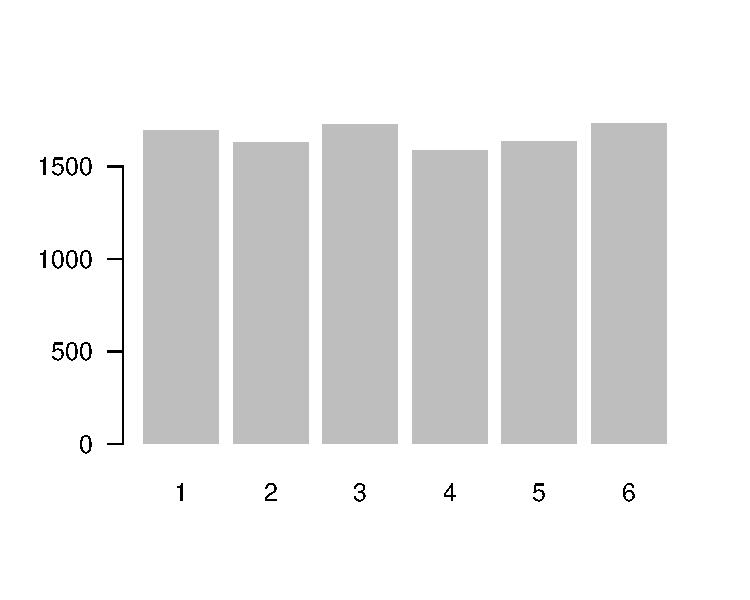
\includegraphics[width=.7\linewidth,height=.6\linewidth]{figure/unnamed-chunk-14-1} 

}



\end{knitrout}

\end{frame}

%------------------------------------------------

\begin{frame}
\begin{center}
\Large{\mdlit{How to simulate a \textbf{loaded} die?}}
\end{center}
\end{frame}

%------------------------------------------------

\begin{frame}[fragile]
\frametitle{Loaded Die}

Changing argument {\hilit \code{prob}} to create a loaded die
\begin{knitrout}\footnotesize
\definecolor{shadecolor}{rgb}{0.969, 0.969, 0.969}\color{fgcolor}\begin{kframe}
\begin{alltt}
\hlstd{probs} \hlkwb{<-} \hlkwd{c}\hlstd{(}\hlnum{1}\hlopt{/}\hlnum{21}\hlstd{,} \hlnum{2}\hlopt{/}\hlnum{21}\hlstd{,}\hlnum{3}\hlopt{/}\hlnum{21}\hlstd{,} \hlnum{4}\hlopt{/}\hlnum{21}\hlstd{,} \hlnum{5}\hlopt{/}\hlnum{21}\hlstd{,} \hlnum{6}\hlopt{/}\hlnum{21}\hlstd{)}

\hlcom{# function}
\hlstd{loaded} \hlkwb{<-} \hlkwa{function}\hlstd{() \{}
  \hlstd{die} \hlkwb{<-} \hlnum{1}\hlopt{:}\hlnum{6}
  \hlkwd{sample}\hlstd{(die,} \hlkwc{size} \hlstd{=} \hlnum{1}\hlstd{,} \hlkwc{prob} \hlstd{= probs)}
\hlstd{\}}
\end{alltt}
\end{kframe}
\end{knitrout}

\pause
\begin{knitrout}\footnotesize
\definecolor{shadecolor}{rgb}{0.969, 0.969, 0.969}\color{fgcolor}\begin{kframe}
\begin{alltt}
\hlkwd{loaded}\hlstd{()}
\end{alltt}
\begin{verbatim}
## [1] 6
\end{verbatim}
\end{kframe}
\end{knitrout}
\end{frame}

%------------------------------------------------

\begin{frame}[fragile]
\frametitle{Rolling a loaded die}
\begin{knitrout}\footnotesize
\definecolor{shadecolor}{rgb}{0.969, 0.969, 0.969}\color{fgcolor}\begin{kframe}
\begin{alltt}
\hlcom{# roll 10 times}
\hlkwa{for} \hlstd{(i} \hlkwa{in} \hlnum{1}\hlopt{:}\hlnum{10}\hlstd{) \{}
  \hlkwd{print}\hlstd{(}\hlkwd{loaded}\hlstd{())}
\hlstd{\}}
\end{alltt}
\begin{verbatim}
## [1] 6
## [1] 5
## [1] 4
## [1] 2
## [1] 6
## [1] 2
## [1] 2
## [1] 4
## [1] 4
## [1] 6
\end{verbatim}
\end{kframe}
\end{knitrout}

\end{frame}

%------------------------------------------------

\begin{frame}[fragile]
\frametitle{Rolling a loaded die}
\begin{knitrout}\footnotesize
\definecolor{shadecolor}{rgb}{0.969, 0.969, 0.969}\color{fgcolor}\begin{kframe}
\begin{alltt}
\hlcom{# roll 10,000 times}
\hlstd{results} \hlkwb{<-} \hlkwd{numeric}\hlstd{(}\hlnum{10000}\hlstd{)}

\hlkwa{for} \hlstd{(i} \hlkwa{in} \hlnum{1}\hlopt{:}\hlnum{10000}\hlstd{) \{}
  \hlstd{results[i]} \hlkwb{<-} \hlkwd{loaded}\hlstd{()}
\hlstd{\}}
\end{alltt}
\end{kframe}
\end{knitrout}

\end{frame}

%------------------------------------------------

\begin{frame}[fragile]
\frametitle{Rolling a lodade die}
\begin{knitrout}\footnotesize
\definecolor{shadecolor}{rgb}{0.969, 0.969, 0.969}\color{fgcolor}\begin{kframe}
\begin{alltt}
\hlcom{# frequencies}
\hlkwd{table}\hlstd{(results)}
\end{alltt}
\begin{verbatim}
## results
##    1    2    3    4    5    6 
##  505 1000 1405 1817 2391 2882
\end{verbatim}
\begin{alltt}
\hlcom{# relative frequencies}
\hlkwd{table}\hlstd{(results)} \hlopt{/} \hlnum{10000}
\end{alltt}
\begin{verbatim}
## results
##      1      2      3      4      5      6 
## 0.0505 0.1000 0.1405 0.1817 0.2391 0.2882
\end{verbatim}
\end{kframe}
\end{knitrout}

\end{frame}

%------------------------------------------------

\begin{frame}[fragile]
\frametitle{Loaded Distribution}

\begin{knitrout}\footnotesize
\definecolor{shadecolor}{rgb}{0.969, 0.969, 0.969}\color{fgcolor}

{\centering 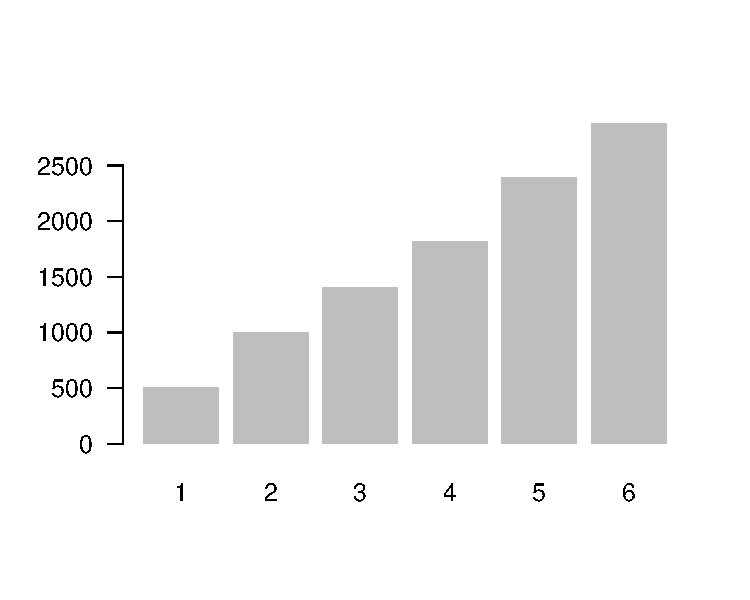
\includegraphics[width=.7\linewidth,height=.6\linewidth]{figure/unnamed-chunk-20-1} 

}



\end{knitrout}

\end{frame}

%------------------------------------------------

\begin{frame}
\begin{center}
\Huge{\hilit{Simulating rolling a pair of dice}}
\end{center}
\end{frame}

%------------------------------------------------

\begin{frame}[fragile]
\frametitle{}
\begin{center}
\ig[width=8cm]{images/dice2.jpg}
\end{center}
\end{frame}

%------------------------------------------------

\begin{frame}[fragile]
\frametitle{Roll a pair of dice}

\begin{knitrout}\footnotesize
\definecolor{shadecolor}{rgb}{0.969, 0.969, 0.969}\color{fgcolor}\begin{kframe}
\begin{alltt}
\hlcom{# 1st die}
\hlkwd{sample}\hlstd{(die,} \hlkwc{size} \hlstd{=} \hlnum{1}\hlstd{)}
\end{alltt}
\begin{verbatim}
## [1] 1
\end{verbatim}
\begin{alltt}
\hlcom{# 2nd die}
\hlkwd{sample}\hlstd{(die,} \hlkwc{size} \hlstd{=} \hlnum{1}\hlstd{)}
\end{alltt}
\begin{verbatim}
## [1] 5
\end{verbatim}
\end{kframe}
\end{knitrout}

\end{frame}

%------------------------------------------------

\begin{frame}[fragile]
\frametitle{Function: roll a pair of dice}

\begin{knitrout}\footnotesize
\definecolor{shadecolor}{rgb}{0.969, 0.969, 0.969}\color{fgcolor}\begin{kframe}
\begin{alltt}
\hlcom{# pair of dice function}
\hlstd{roll2} \hlkwb{<-} \hlkwa{function}\hlstd{() \{}




\hlstd{\}}
\end{alltt}
\end{kframe}
\end{knitrout}

\end{frame}

%------------------------------------------------

\begin{frame}[fragile]
\frametitle{Function: roll a pair of dice}

\begin{knitrout}\footnotesize
\definecolor{shadecolor}{rgb}{0.969, 0.969, 0.969}\color{fgcolor}\begin{kframe}
\begin{alltt}
\hlcom{# pair of dice function}
\hlstd{roll2} \hlkwb{<-} \hlkwa{function}\hlstd{() \{}
  \hlstd{die} \hlkwb{<-} \hlnum{1}\hlopt{:}\hlnum{6}
  \hlstd{rol1} \hlkwb{<-} \hlkwd{sample}\hlstd{(die,} \hlkwc{size} \hlstd{=} \hlnum{1}\hlstd{)}
  \hlstd{rol2} \hlkwb{<-} \hlkwd{sample}\hlstd{(die,} \hlkwc{size} \hlstd{=} \hlnum{1}\hlstd{)}
  \hlkwd{c}\hlstd{(rol1, rol2)}
\hlstd{\}}
\end{alltt}
\end{kframe}
\end{knitrout}

\end{frame}

%------------------------------------------------

\begin{frame}[fragile]
\frametitle{Various rolls}

\begin{knitrout}\footnotesize
\definecolor{shadecolor}{rgb}{0.969, 0.969, 0.969}\color{fgcolor}\begin{kframe}
\begin{alltt}
\hlkwd{roll2}\hlstd{()}
\end{alltt}
\begin{verbatim}
## [1] 5 1
\end{verbatim}
\begin{alltt}
\hlkwd{roll2}\hlstd{()}
\end{alltt}
\begin{verbatim}
## [1] 1 1
\end{verbatim}
\begin{alltt}
\hlkwd{roll2}\hlstd{()}
\end{alltt}
\begin{verbatim}
## [1] 6 6
\end{verbatim}
\end{kframe}
\end{knitrout}

\end{frame}

%------------------------------------------------

\begin{frame}[fragile]
\frametitle{Function}

\begin{knitrout}\footnotesize
\definecolor{shadecolor}{rgb}{0.969, 0.969, 0.969}\color{fgcolor}\begin{kframe}
\begin{alltt}
\hlcom{# pair of dice function}
\hlstd{roll2} \hlkwb{<-} \hlkwa{function}\hlstd{() \{}
  \hlstd{die} \hlkwb{<-} \hlnum{1}\hlopt{:}\hlnum{6}
  \hlstd{rol1} \hlkwb{<-} \hlkwd{sample}\hlstd{(die,} \hlkwc{size} \hlstd{=} \hlnum{1}\hlstd{)}
  \hlstd{rol2} \hlkwb{<-} \hlkwd{sample}\hlstd{(die,} \hlkwc{size} \hlstd{=} \hlnum{1}\hlstd{)}  \hlcom{# repeated command!}
  \hlkwd{c}\hlstd{(rol1, rol2)}
\hlstd{\}}
\end{alltt}
\end{kframe}
\end{knitrout}

\end{frame}

%------------------------------------------------

\begin{frame}[fragile]
\frametitle{Roll a pair of dice}

\begin{knitrout}\footnotesize
\definecolor{shadecolor}{rgb}{0.969, 0.969, 0.969}\color{fgcolor}\begin{kframe}
\begin{alltt}
\hlstd{die} \hlkwb{<-} \hlnum{1}\hlopt{:}\hlnum{6}

\hlcom{# avoid repetition with one call of 'sample()'}
\hlkwd{sample}\hlstd{(die,} \hlkwc{size} \hlstd{=} \hlnum{2}\hlstd{)}
\end{alltt}
\begin{verbatim}
## [1] 6 1
\end{verbatim}
\end{kframe}
\end{knitrout}

\end{frame}

%------------------------------------------------

\begin{frame}[fragile]
\frametitle{Roll a pair dice}

\begin{knitrout}\scriptsize
\definecolor{shadecolor}{rgb}{0.969, 0.969, 0.969}\color{fgcolor}\begin{kframe}
\begin{alltt}
\hlkwa{for} \hlstd{(i} \hlkwa{in} \hlnum{1}\hlopt{:}\hlnum{15}\hlstd{) \{}
  \hlkwd{print}\hlstd{(}\hlkwd{sample}\hlstd{(die,} \hlkwc{size} \hlstd{=} \hlnum{2}\hlstd{))}
\hlstd{\}}
\end{alltt}
\begin{verbatim}
## [1] 1 3
## [1] 1 4
## [1] 5 4
## [1] 4 3
## [1] 3 1
## [1] 2 6
## [1] 4 6
## [1] 3 4
## [1] 4 6
## [1] 6 3
## [1] 2 5
## [1] 2 5
## [1] 2 3
## [1] 3 2
## [1] 2 5
\end{verbatim}
\begin{alltt}
\hlcom{# Can you spot a problem?}
\end{alltt}
\end{kframe}
\end{knitrout}

\end{frame}

%------------------------------------------------

\begin{frame}[fragile]
\frametitle{Roll a pair of dice}

\begin{knitrout}\footnotesize
\definecolor{shadecolor}{rgb}{0.969, 0.969, 0.969}\color{fgcolor}\begin{kframe}
\begin{alltt}
\hlstd{die} \hlkwb{<-} \hlnum{1}\hlopt{:}\hlnum{6}

\hlcom{# sample with replacement}
\hlkwd{sample}\hlstd{(die,} \hlkwc{size} \hlstd{=} \hlnum{2}\hlstd{,} \hlkwc{replace} \hlstd{=} \hlnum{TRUE}\hlstd{)}
\end{alltt}
\begin{verbatim}
## [1] 4 1
\end{verbatim}
\end{kframe}
\end{knitrout}

\end{frame}

%------------------------------------------------

\begin{frame}[fragile]
\frametitle{Roll a pair of dice}

\begin{knitrout}\scriptsize
\definecolor{shadecolor}{rgb}{0.969, 0.969, 0.969}\color{fgcolor}\begin{kframe}
\begin{alltt}
\hlkwa{for} \hlstd{(i} \hlkwa{in} \hlnum{1}\hlopt{:}\hlnum{15}\hlstd{) \{}
  \hlkwd{print}\hlstd{(}\hlkwd{sample}\hlstd{(die,} \hlkwc{size} \hlstd{=} \hlnum{2}\hlstd{,} \hlkwc{replace} \hlstd{=} \hlnum{TRUE}\hlstd{))}
\hlstd{\}}
\end{alltt}
\begin{verbatim}
## [1] 6 6
## [1] 6 5
## [1] 5 4
## [1] 3 6
## [1] 1 2
## [1] 1 5
## [1] 1 2
## [1] 3 1
## [1] 6 1
## [1] 1 2
## [1] 1 6
## [1] 3 2
## [1] 3 1
## [1] 2 2
## [1] 1 1
\end{verbatim}
\end{kframe}
\end{knitrout}
\end{frame}

%------------------------------------------------

\begin{frame}[fragile]
\frametitle{Roll a pair of dice}

\begin{knitrout}\footnotesize
\definecolor{shadecolor}{rgb}{0.969, 0.969, 0.969}\color{fgcolor}\begin{kframe}
\begin{alltt}
\hlcom{# rewrite roll2()}
\hlstd{roll2} \hlkwb{<-} \hlkwa{function}\hlstd{() \{}
  \hlstd{die} \hlkwb{<-} \hlnum{1}\hlopt{:}\hlnum{6}
  \hlkwd{sample}\hlstd{(die,} \hlkwc{size} \hlstd{=} \hlnum{2}\hlstd{,} \hlkwc{replace} \hlstd{=} \hlnum{TRUE}\hlstd{)}
\hlstd{\}}
\end{alltt}
\end{kframe}
\end{knitrout}

\pause
\begin{knitrout}\footnotesize
\definecolor{shadecolor}{rgb}{0.969, 0.969, 0.969}\color{fgcolor}\begin{kframe}
\begin{alltt}
\hlkwd{roll2}\hlstd{()}
\end{alltt}
\begin{verbatim}
## [1] 5 4
\end{verbatim}
\end{kframe}
\end{knitrout}
\end{frame}

%------------------------------------------------

\begin{frame}
\begin{center}
\Huge{\hilit{Rolling a die any number of times}}
\end{center}
\end{frame}

%------------------------------------------------

\begin{frame}[fragile]
\frametitle{Rolling several dice}

More general function to roll a die any number of times
\begin{knitrout}\footnotesize
\definecolor{shadecolor}{rgb}{0.969, 0.969, 0.969}\color{fgcolor}\begin{kframe}
\begin{alltt}
\hlstd{roll} \hlkwb{<-} \hlkwa{function}\hlstd{(}\hlkwc{times} \hlstd{=} \hlnum{1}\hlstd{) \{}
  \hlstd{die} \hlkwb{<-} \hlnum{1}\hlopt{:}\hlnum{6}
  \hlkwd{sample}\hlstd{(die,} \hlkwc{size} \hlstd{= times,} \hlkwc{replace} \hlstd{=} \hlnum{TRUE}\hlstd{)}
\hlstd{\}}
\end{alltt}
\end{kframe}
\end{knitrout}

\pause
\begin{knitrout}\footnotesize
\definecolor{shadecolor}{rgb}{0.969, 0.969, 0.969}\color{fgcolor}\begin{kframe}
\begin{alltt}
\hlkwd{roll}\hlstd{()}
\end{alltt}
\begin{verbatim}
## [1] 4
\end{verbatim}
\end{kframe}
\end{knitrout}
\end{frame}

%------------------------------------------------

\begin{frame}[fragile]
\frametitle{Rolling several dice}

\begin{knitrout}\footnotesize
\definecolor{shadecolor}{rgb}{0.969, 0.969, 0.969}\color{fgcolor}\begin{kframe}
\begin{alltt}
\hlcom{# default (one roll)}
\hlkwd{roll}\hlstd{()}
\end{alltt}
\begin{verbatim}
## [1] 4
\end{verbatim}
\begin{alltt}
\hlcom{# two rolls}
\hlkwd{roll}\hlstd{(}\hlnum{2}\hlstd{)}
\end{alltt}
\begin{verbatim}
## [1] 1 5
\end{verbatim}
\begin{alltt}
\hlcom{# 4 rolls }
\hlkwd{roll}\hlstd{(}\hlnum{4}\hlstd{)}
\end{alltt}
\begin{verbatim}
## [1] 6 4 6 5
\end{verbatim}
\end{kframe}
\end{knitrout}
\end{frame}

%------------------------------------------------

\begin{frame}
\begin{center}
\Huge{\hilit{De Mere's Game 1}}
\end{center}
\end{frame}

%------------------------------------------------

\begin{frame}[fragile]
\frametitle{De Mere's Game 1}

\bb{Game 1}
\bi
  \item One die
  \item Four rolls
  \item Win: at least one 6
\ei
\eb

\end{frame}

%------------------------------------------------

\begin{frame}[fragile]
\frametitle{De Mere's Game 1}

\begin{knitrout}\footnotesize
\definecolor{shadecolor}{rgb}{0.969, 0.969, 0.969}\color{fgcolor}\begin{kframe}
\begin{alltt}
\hlcom{# play 100 times}
\hlstd{results} \hlkwb{<-} \hlkwd{matrix}\hlstd{(}\hlnum{0}\hlstd{,} \hlkwc{nrow} \hlstd{=} \hlnum{100}\hlstd{,} \hlkwc{ncol} \hlstd{=} \hlnum{4}\hlstd{)}

\hlkwa{for} \hlstd{(i} \hlkwa{in} \hlnum{1}\hlopt{:}\hlnum{100}\hlstd{) \{}
  \hlstd{results[i, ]} \hlkwb{<-} \hlkwd{roll}\hlstd{(}\hlkwc{times} \hlstd{=} \hlnum{4}\hlstd{)}
\hlstd{\}}

\hlkwd{head}\hlstd{(results)}
\end{alltt}
\begin{verbatim}
##      [,1] [,2] [,3] [,4]
## [1,]    2    5    4    2
## [2,]    6    6    1    6
## [3,]    3    4    4    2
## [4,]    5    2    3    6
## [5,]    6    2    3    1
## [6,]    4    3    6    1
\end{verbatim}
\end{kframe}
\end{knitrout}

\end{frame}

%------------------------------------------------

\begin{frame}[fragile]
\frametitle{De Mere's Game 1}

\begin{knitrout}\footnotesize
\definecolor{shadecolor}{rgb}{0.969, 0.969, 0.969}\color{fgcolor}\begin{kframe}
\begin{alltt}
\hlstd{counts} \hlkwb{<-} \hlnum{0}

\hlkwa{for} \hlstd{(i} \hlkwa{in} \hlnum{1}\hlopt{:}\hlnum{100}\hlstd{) \{}
  \hlkwa{if} \hlstd{(}\hlkwd{any}\hlstd{(results[i, ]} \hlopt{==} \hlnum{6}\hlstd{))}
    \hlstd{counts} \hlkwb{<-} \hlstd{counts} \hlopt{+} \hlnum{1}
\hlstd{\}}

\hlcom{# proportion of wins}
\hlstd{counts} \hlopt{/} \hlnum{100}
\end{alltt}
\begin{verbatim}
## [1] 0.56
\end{verbatim}
\end{kframe}
\end{knitrout}

\end{frame}

%------------------------------------------------

\begin{frame}[fragile]
\frametitle{De Mere's Game 1}

\begin{knitrout}\footnotesize
\definecolor{shadecolor}{rgb}{0.969, 0.969, 0.969}\color{fgcolor}\begin{kframe}
\begin{alltt}
\hlstd{sixes} \hlkwb{<-} \hlkwd{apply}\hlstd{(results,} \hlnum{1}\hlstd{,} \hlkwa{function}\hlstd{(}\hlkwc{x}\hlstd{)} \hlkwd{sum}\hlstd{(x} \hlopt{==} \hlnum{6}\hlstd{))}

\hlkwd{table}\hlstd{(sixes)}
\end{alltt}
\begin{verbatim}
## sixes
##  0  1  2  3 
## 44 41 13  2
\end{verbatim}
\end{kframe}
\end{knitrout}

\pause
\begin{knitrout}\footnotesize
\definecolor{shadecolor}{rgb}{0.969, 0.969, 0.969}\color{fgcolor}\begin{kframe}
\begin{alltt}
\hlcom{# rolls with at least one six}
\hlkwd{sum}\hlstd{(}\hlkwd{table}\hlstd{(sixes)[}\hlopt{-}\hlnum{1}\hlstd{])}
\end{alltt}
\begin{verbatim}
## [1] 56
\end{verbatim}
\end{kframe}
\end{knitrout}

\end{frame}

%------------------------------------------------

\begin{frame}[fragile]
\frametitle{De Mere's Game 1}

\begin{knitrout}\footnotesize
\definecolor{shadecolor}{rgb}{0.969, 0.969, 0.969}\color{fgcolor}

{\centering 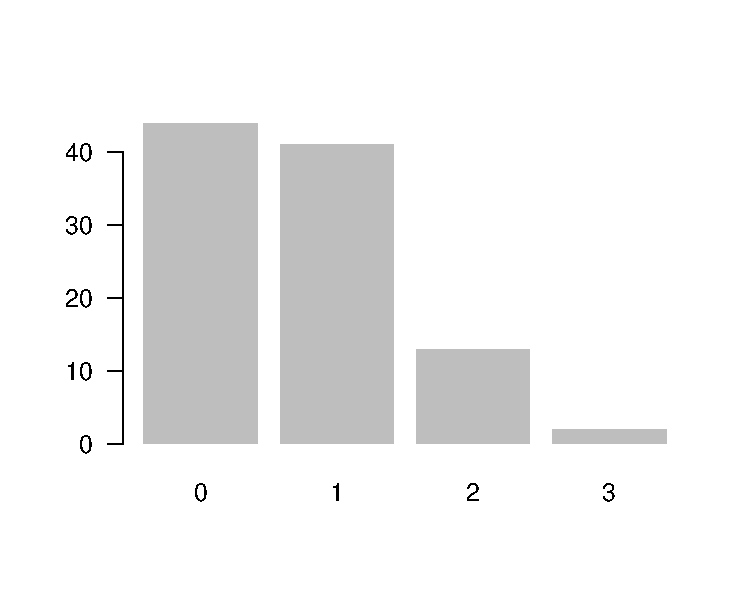
\includegraphics[width=.7\linewidth,height=.6\linewidth]{figure/unnamed-chunk-39-1} 

}



\end{knitrout}

\end{frame}

%------------------------------------------------

\begin{frame}[fragile]
\frametitle{De Mere's Game 1}

\bb{Considerations}
\bbi
  \item How would you make the code more flexible?
  \item What type of ``parameters''?
  \item Avoid Repetition
\ei
\eb

\end{frame}

%------------------------------------------------

\begin{frame}[fragile]
\frametitle{De Mere's Game 1}

\begin{knitrout}\footnotesize
\definecolor{shadecolor}{rgb}{0.969, 0.969, 0.969}\color{fgcolor}\begin{kframe}
\begin{alltt}
\hlstd{games} \hlkwb{<-} \hlnum{10000}
\hlstd{results} \hlkwb{<-} \hlkwd{matrix}\hlstd{(}\hlnum{0}\hlstd{,} \hlkwc{nrow} \hlstd{= games,} \hlkwc{ncol} \hlstd{=} \hlnum{4}\hlstd{)}

\hlkwa{for} \hlstd{(i} \hlkwa{in} \hlnum{1}\hlopt{:}\hlstd{games) \{}
  \hlstd{results[i, ]} \hlkwb{<-} \hlkwd{roll}\hlstd{(}\hlkwc{times} \hlstd{=} \hlnum{4}\hlstd{)}
\hlstd{\}}

\hlstd{counts} \hlkwb{<-} \hlnum{0}
\hlkwa{for} \hlstd{(i} \hlkwa{in} \hlnum{1}\hlopt{:}\hlstd{games) \{}
  \hlkwa{if} \hlstd{(}\hlkwd{any}\hlstd{(results[i, ]} \hlopt{==} \hlnum{6}\hlstd{))}
    \hlstd{counts} \hlkwb{<-} \hlstd{counts} \hlopt{+} \hlnum{1}
\hlstd{\}}

\hlstd{counts} \hlopt{/} \hlstd{games}  \hlcom{# proportion of wins}
\end{alltt}
\begin{verbatim}
## [1] 0.5204
\end{verbatim}
\end{kframe}
\end{knitrout}

\end{frame}

%------------------------------------------------

\begin{frame}[fragile]
\frametitle{De Mere's Game 1}

\begin{knitrout}\footnotesize
\definecolor{shadecolor}{rgb}{0.969, 0.969, 0.969}\color{fgcolor}\begin{kframe}
\begin{alltt}
\hlstd{sixes} \hlkwb{<-} \hlkwd{apply}\hlstd{(results,} \hlnum{1}\hlstd{,} \hlkwa{function}\hlstd{(}\hlkwc{x}\hlstd{)} \hlkwd{sum}\hlstd{(x} \hlopt{==} \hlnum{6}\hlstd{))}

\hlkwd{table}\hlstd{(sixes)}
\end{alltt}
\begin{verbatim}
## sixes
##    0    1    2    3    4 
## 4796 3858 1171  166    9
\end{verbatim}
\end{kframe}
\end{knitrout}

\pause
\begin{knitrout}\footnotesize
\definecolor{shadecolor}{rgb}{0.969, 0.969, 0.969}\color{fgcolor}\begin{kframe}
\begin{alltt}
\hlcom{# rolls with at least one six}
\hlkwd{sum}\hlstd{(}\hlkwd{table}\hlstd{(sixes)[}\hlopt{-}\hlnum{1}\hlstd{])}
\end{alltt}
\begin{verbatim}
## [1] 5204
\end{verbatim}
\end{kframe}
\end{knitrout}

\end{frame}

%------------------------------------------------

\begin{frame}[fragile]
\frametitle{De Mere's Game 1}

\begin{knitrout}\footnotesize
\definecolor{shadecolor}{rgb}{0.969, 0.969, 0.969}\color{fgcolor}

{\centering 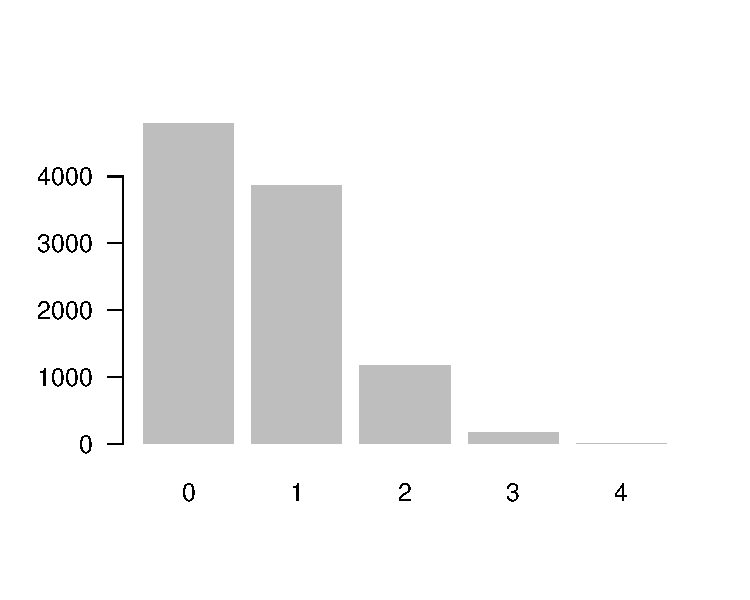
\includegraphics[width=.7\linewidth,height=.6\linewidth]{figure/unnamed-chunk-43-1} 

}



\end{knitrout}

\end{frame}

%------------------------------------------------

\begin{frame}
\begin{center}
\Huge{\hilit{De Mere's Game 2}}
\end{center}
\end{frame}

%------------------------------------------------

\begin{frame}[fragile]
\frametitle{De Mere's Game 2}

\bb{Game 2}
\bi
  \item Two dice
  \item 24 rolls
  \item Win: at least one double 6
\ei
\eb

\end{frame}

%------------------------------------------------

\begin{frame}[fragile]
\frametitle{De Mere's Game 2}

\begin{knitrout}\footnotesize
\definecolor{shadecolor}{rgb}{0.969, 0.969, 0.969}\color{fgcolor}\begin{kframe}
\begin{alltt}
\hlstd{roll2} \hlkwb{<-} \hlkwa{function}\hlstd{(}\hlkwc{times} \hlstd{=} \hlnum{1}\hlstd{) \{}
  \hlstd{dice2} \hlkwb{<-} \hlkwd{unlist}\hlstd{(}\hlkwd{lapply}\hlstd{(}\hlnum{1}\hlopt{:}\hlnum{6}\hlstd{,} \hlkwa{function}\hlstd{(}\hlkwc{x}\hlstd{) x} \hlopt{+} \hlnum{1}\hlopt{:}\hlnum{6}\hlstd{))}
  \hlkwd{sample}\hlstd{(dice2,} \hlkwc{size} \hlstd{= times,} \hlkwc{replace} \hlstd{=} \hlnum{TRUE}\hlstd{)}
\hlstd{\}}

\hlkwd{roll2}\hlstd{()}
\end{alltt}
\begin{verbatim}
## [1] 10
\end{verbatim}
\begin{alltt}
\hlkwd{roll2}\hlstd{(}\hlnum{24}\hlstd{)}
\end{alltt}
\begin{verbatim}
##  [1]  8  4  4  3  8  6  7  6  9  9  5  4  5  7  3 11  9 11 10  8  9  4 11  6
\end{verbatim}
\end{kframe}
\end{knitrout}
\end{frame}

%------------------------------------------------

\begin{frame}[fragile]
\frametitle{De Mere's Game 2}

\bb{Game 2}
\bbi
  \item It's better if we sum the points of rolling two dice
  \item Possible outcomes: $\{2, 3, 4, \dots, 10, 11, 12\}$
  \item Double six is equivalent to 12 points
\ei
\eb

\end{frame}

%------------------------------------------------

\begin{frame}[fragile]
\frametitle{De Mere's Game 2}

\begin{knitrout}\footnotesize
\definecolor{shadecolor}{rgb}{0.969, 0.969, 0.969}\color{fgcolor}\begin{kframe}
\begin{alltt}
\hlstd{games} \hlkwb{<-} \hlnum{10000}
\hlstd{results} \hlkwb{<-} \hlkwd{matrix}\hlstd{(}\hlnum{0}\hlstd{,} \hlkwc{nrow} \hlstd{= games,} \hlkwc{ncol} \hlstd{=} \hlnum{24}\hlstd{)}

\hlkwa{for} \hlstd{(i} \hlkwa{in} \hlnum{1}\hlopt{:}\hlstd{games) \{}
  \hlstd{results[i, ]} \hlkwb{<-} \hlkwd{roll2}\hlstd{(}\hlnum{24}\hlstd{)}
\hlstd{\}}

\hlstd{doublesix} \hlkwb{<-} \hlkwd{apply}\hlstd{(results,} \hlnum{1}\hlstd{,} \hlkwa{function}\hlstd{(}\hlkwc{x}\hlstd{)} \hlkwd{sum}\hlstd{(x} \hlopt{==} \hlnum{12}\hlstd{))}

\hlkwd{sum}\hlstd{(}\hlkwd{table}\hlstd{(doublesix)[}\hlopt{-}\hlnum{1}\hlstd{])}
\end{alltt}
\begin{verbatim}
## [1] 4930
\end{verbatim}
\end{kframe}
\end{knitrout}

\end{frame}

%------------------------------------------------

\begin{frame}[fragile]
\frametitle{De Mere's Game 2}

\begin{knitrout}\footnotesize
\definecolor{shadecolor}{rgb}{0.969, 0.969, 0.969}\color{fgcolor}

{\centering 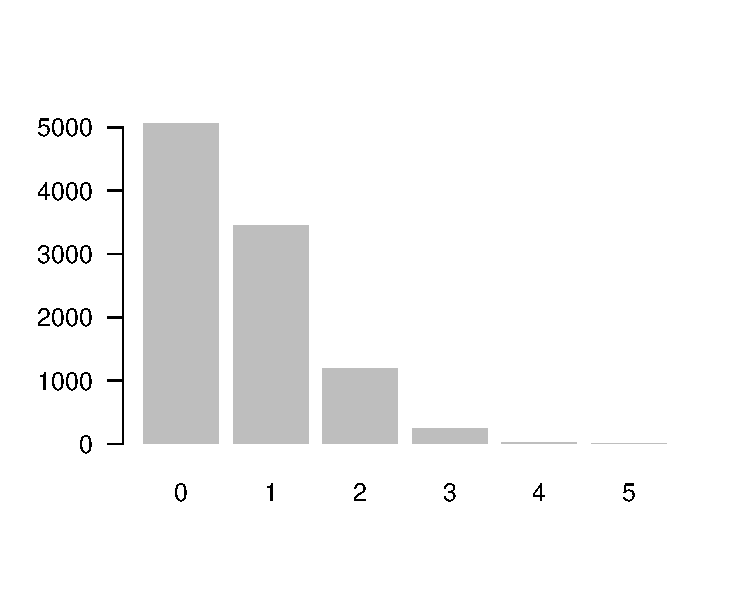
\includegraphics[width=.7\linewidth,height=.6\linewidth]{figure/unnamed-chunk-46-1} 

}



\end{knitrout}

\end{frame}

%------------------------------------------------

\begin{frame}[fragile]
\frametitle{De Mere's Game 2}

\begin{knitrout}\footnotesize
\definecolor{shadecolor}{rgb}{0.969, 0.969, 0.969}\color{fgcolor}\begin{kframe}
\begin{alltt}
\hlstd{counts} \hlkwb{<-} \hlnum{0}
\hlkwa{for} \hlstd{(i} \hlkwa{in} \hlnum{1}\hlopt{:}\hlstd{games) \{}
  \hlkwa{if} \hlstd{(}\hlkwd{any}\hlstd{(results[i, ]} \hlopt{==} \hlnum{12}\hlstd{))}
    \hlstd{counts} \hlkwb{<-} \hlstd{counts} \hlopt{+} \hlnum{1}
\hlstd{\}}

\hlstd{counts} \hlopt{/} \hlstd{games}  \hlcom{# proportion of wins}
\end{alltt}
\begin{verbatim}
## [1] 0.493
\end{verbatim}
\end{kframe}
\end{knitrout}

\end{frame}

%------------------------------------------------

\end{document}
